
\documentclass[dvipdfmx]{standalone}
\usepackage[T1]{fontenc}
\usepackage{newtxtext, newtxmath}

\usepackage{tikz}
\usetikzlibrary{circuits.logic.CDH}

\begin{document}
  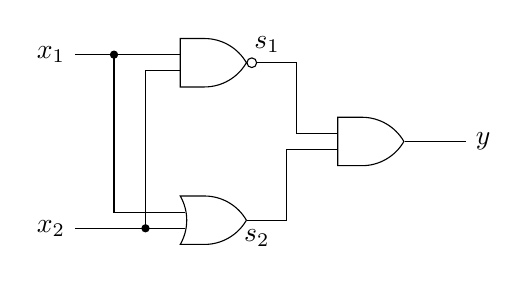
\begin{tikzpicture}[circuit logic CDH]
    \tikzset{branch/.style={fill, shape=circle, minimum size=3pt, inner sep=0pt}}

    \draw (2,2) node (f1) [nand gate] {};
    \draw (2,0) node (f2) [or gate] {};
    \draw (4,1) node (f3) [and gate] {};

    \draw[opacity=0] (0,0) -- (up:1mm) node (y axis) {};
    \draw (f1.input 1 -| y axis) node (x1) {$x_1$};
    \draw (f2.input 2 -| y axis) node (x2) {$x_2$};
    \draw (f3.output) ++(1,0) node (y) {$y$};

    \draw (x1) -- (f1.input 1);
    \draw (x2) -- (f2.input 2);
    \draw (x1) ++(0.8,0) node[branch]{} |- (f2.input 1);
    \draw (x2) ++(1.2,0) node[branch]{} |- (f1.input 2);
    \draw (f1.output) -- node[above, near start] {$s_1$} ++(0.5,0) |- (f3.input 1);
    \draw (f2.output) -- node[below, near start] {$s_2$} ++(0.5,0) |- (f3.input 2);
    \draw (f3.output) -- (y);
  \end{tikzpicture}
\end{document}
